\section{Tree Editor}\label{sec:result-tree-editor}

This section will present the findings for a \emph{Tree Editor}.

\subsection{Functional requirements for final editor}

Here is a list of identified requirements.
Note that it may not be complete, with regards to usability and all possible features for \gls{mdd} tools.
More requirements should be specified for a final product, in further works.
A good source for requirements are the existing editors mentioned in \cref{sec:ecore-editors}, with regards to a complete solution with good usability.

% Please add the following required packages to your document preamble:
% \usepackage{longtable}
% Note: It may be necessary to compile the document several times to get a multi-page table to line up properly
\begin{longtable}{lp{3cm}p{6cm}}
\caption{Functional requirements for a master-detail Tree editor with property sheet.}
\label{tab:function-requirements}\\
\multicolumn{1}{c}{\textbf{ID}} &
  \multicolumn{1}{c}{\textbf{Requirement}} &
  \multicolumn{1}{c}{\textbf{Description}} \\ \hline
\endfirsthead
%
\multicolumn{3}{c}%
{{\bfseries Table \thetable\ continued from previous page}} \\
\multicolumn{1}{c}{\textbf{ID}} &
  \multicolumn{1}{c}{\textbf{Requirement}} &
  \multicolumn{1}{c}{\textbf{Description}} \\ \hline
\endhead
%
FR1 &
  Provide an interactive Tree Editor in VSCode and Theia (Gitpod) &
  \begin{tabular}[c]{@{}p{6cm}@{}}The software must use an extension mechanism to provide a custom editor for trees.\\ A textual representation is not sufficient.\\ The tree comprises a hierarchy of nodes and their child nodes.\end{tabular} \\
FR2 &
  Provide an interactive Property sheet in VSCode and Theia (Gitpod) &
  \begin{tabular}[c]{@{}p{6cm}@{}}The software must use an extension mechanism to provide a custom property sheet for tree nodes.\\ The property sheet needs to be synchronized with the selected node in the tree editor.\end{tabular} \\
FR3 &
  Provide an action bar with dynamically provided actions in VSCode and Theia (Gitpod). &
  The action bar should have actions that are specified by a backend Tree Language Server. \\
FR4 &
  The Tree must view nodes with labels and icons. &
  \begin{tabular}[c]{@{}p{6cm}@{}}Every node should have a default icon that depends on its node "type".\\ Every node should have a name that is read from the node data.\end{tabular} \\
FR5 &
  Tree nodes with children can toggle the visibility of children by user interaction. &
  \begin{tabular}[c]{@{}p{6cm}@{}}An icon or symbol will show if a node has children.\\ If the user interacts with this icon, e.g. a click, all the children will toggle their visibility on/off.\end{tabular} \\
FR6 &
  The Tree and Property views update automatically when the underlying model changes. &
  Subscribe to change notifications from the Model Server, in the Tree Language Server. \\
FR7 &
  The Action Bar updates when the tree selection changes. &
  Show the available actions for the newly selected node. \\
FR8 &
  Support creation of new nodes. &
   \\
FR9 &
  Support deletion of existing nodes. &
   \\
FR10 &
  Support selecting a node. &
   \\
 &
   &
  
\end{longtable} %TODO: make sure table is not clipping


\subsection{Architecture and protocols}

A suggestion for an architecture is to use an \emph{VSCode extension} with a \emph{WebView} and \emph{CustomEditor}.
Connect the extension to a bundled \emph{Tree Language Server} by using \gls{JSON-RPC} or \gls{REST} and \gls{WebSocket}.
The transport mechanism between the extension and the Tree Language Server can be either standard input/output (stdio) or TCP sockets.
The Tree Language Server should hold any language dependent details, like mappings from \gls{Ecore} over to a generic tree structure.
Any changes to the model should be relayed from the extension via the Tree Language Server to the Model Server.
The extension should only talk about changes in a general manner with the Tree Language Server.
These will be converted to \gls{Ecore} specific operations in the Tree Language Server before being sent to the Model Server over a \gls{REST} \acrshort{API}.
A diagram with this architecture is shown in \cref{fig:tree-editor-architecture}.

\begin{figure}[htbp]
  \centering
  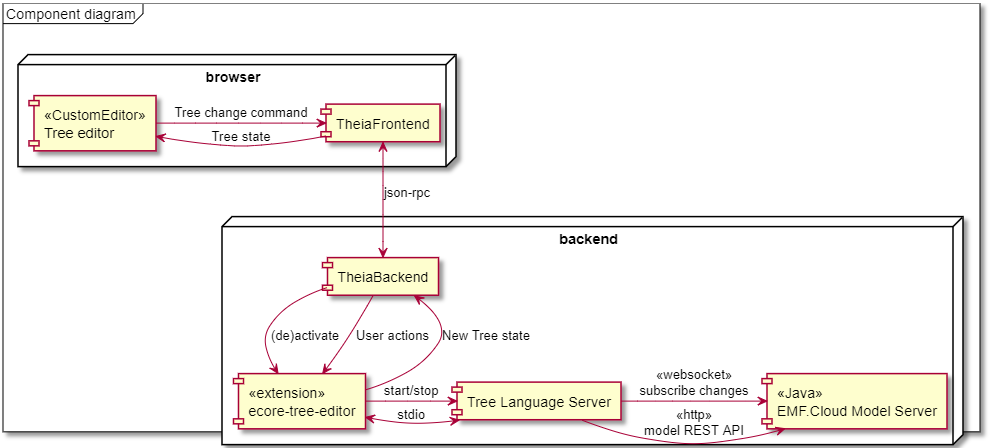
\includegraphics[width=\textwidth]{figures/tree-editor-component-diagram.png}
  \caption[Tree Editor Architecture]{A suggested architecture for a tree editor.}\label{fig:tree-editor-architecture}
\end{figure}

\paragraph*{Sharing a Model Server}
Because multiple extensions might require the same Model Server, an idea (not explored yet) is to have a specific VSCode Extension only for providing this Model Server.
Other extensions can then notify a dependence on this extension, causing it to be installed.
This seems supported at least in VSCode.
The Model Server extension would then provide the details for connecting to it, to other extensions.
It is possible to discover other extensions and get an \gls{API} from them.

